% Created 2021-09-10 Fri 12:59
% Intended LaTeX compiler: pdflatex
\documentclass[11pt]{article}
\usepackage[utf8]{inputenc}
\usepackage[T1]{fontenc}
\usepackage{graphicx}
\graphicspath{{./img/}}
\usepackage{grffile}
\usepackage{longtable}

\usepackage[normalem]{ulem}
\usepackage{amsmath}
\usepackage{textcomp}
\usepackage{amssymb}

\usepackage{hyperref}
\date{\today}
\title{}
\hypersetup{
 pdfauthor={},
 pdftitle={},
 pdfkeywords={},
 pdfsubject={},
 pdfcreator={Emacs 27.2 (Org mode 9.4.4)}, 
 pdflang={English}}
\begin{document}

\tableofcontents

\#+title Project 2
\#+author Duncan Wilkie
\#+date\textit{<2021-09-10 Fri>}


\section{Analytical Solution}
\label{sec:orgf4520d7}

We know from the study of Taylor series that \(\sum_{n=0}^\infty\frac{(-x)^n}{n!} = e^{-x}\). 

\section{Numerical Method}
\label{sec:org8e56bb6}

Computationally, we may approximate the infinite sum by using a large number of terms, using tail recursion to keep the computation \(O(n)\).

\section{Program 1}
\label{sec:org517aaca}

\begin{verbatim}

#include <iostream>
#include <fstream>
#include <cmath>

using namespace std;

int main() {
  float error, sum, element, exact, x;

  error = 1e-6;

  cout << "Input a (floating point) number: " << endl;
  cin >> x;

  sum = 1.;
  element = 1.;
  exact = exp(-x);

  int n = 0;
  do {
    ++n;
    element *= -x/n;
    sum += element;
    cout << "n: " << n << ", element: " << element << ", sum: " << sum \
        << ", exact: " << exact << endl;
  } while (sum == 0 || fabs(element / sum) > error);


  return 0;

}

\end{verbatim}

\section{Program 2}
\label{sec:org2b59d8a}

\begin{verbatim}

#include <cmath>
#include <iostream>
#include <fstream>

using namespace std;

int main() {
  float error, xmin, xmax, xstep, sum, element, exact, x;
  ofstream outfile("p2_out.txt");

  error = 1e-6;
  xmin = 0.; xmax = 10.0; xstep = 0.1;

  x = xmin;
  outfile << "n\tx\tsum\texact\tsum-exact" << endl; 
  while (x < xmax + 0.5 * xstep) {
    sum = 1.;
    element = 1.;
    exact = exp(-x);

    int n = 0;
    do {
      ++n;
      element *= -x/n;
      sum += element;
    } while (sum == 0 || fabs(element / sum) > error);


    outfile << n << " " << x << " " << sum << " " << exact \
        << " " << sum - exact << endl;

    x += xstep;
  }

  return 0;

}

\end{verbatim}

\section{Program 1 Analysis}
\label{sec:orgdb0e617}

Graphs of the finite and exact results as a function of \(n\) for $x=0.8$ and $x=10$ appear below.
\[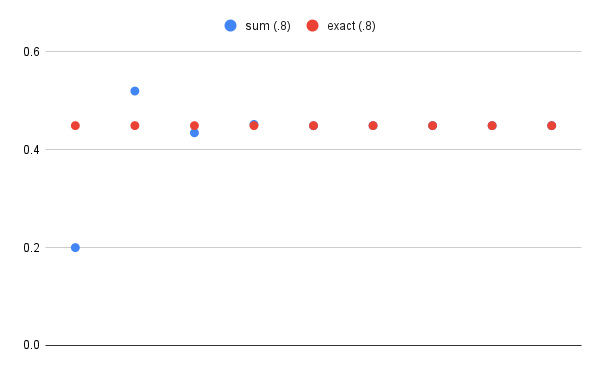
\includegraphics[scale=0.5]{img/chart.png}\]
\[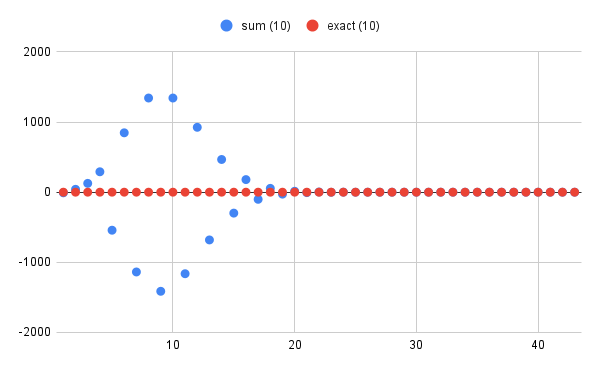
\includegraphics[scale=0.5]{img/chart1.png}\]
Clearly, there is a quick convergence towards the exact solution in this case, with nearly indistinguishable results at \(n=5\) in the first case and $n=20$ in the second.

For \(x=10\), part of the output of Program 1 appears below.

\begin{verbatim}

[dwilk14@tigers ~/Project2]$ ./dwilk14_proj2p1
Input a (floating point) number:
10
n: 1, element: -10, sum: -9, exact: 4.53999e-05
n: 2, element: 50, sum: 41, exact: 4.53999e-05
n: 3, element: -166.667, sum: -125.667, exact: 4.53999e-05
n: 4, element: 416.667, sum: 291, exact: 4.53999e-05
n: 5, element: -833.333, sum: -542.333, exact: 4.53999e-05
n: 6, element: 1388.89, sum: 846.555, exact: 4.53999e-05
n: 7, element: -1984.13, sum: -1137.57, exact: 4.53999e-05
n: 8, element: 2480.16, sum: 1342.59, exact: 4.53999e-05
n: 9, element: -2755.73, sum: -1413.14, exact: 4.53999e-05
n: 10, element: 2755.73, sum: 1342.59, exact: 4.53999e-05
n: 11, element: -2505.21, sum: -1162.62, exact: 4.53999e-05
n: 12, element: 2087.68, sum: 925.052, exact: 4.53999e-05

\end{verbatim}

Comparing \(n=9\) and \(n=10\), we can see that the corresponding terms are large and are almost exactly additive inverses of each other.

For small \(n\), the error is quite high. This is an approximation error, as the sum isn't given sufficient terms to converge very well.

\section{Program 2 Analysis}
\label{sec:orgf7f6b3d}

Below is a plot of the computed and exact solutions as a function of \(x\in[6, 10]\). The two are extremely close; the finite sum is a good approximation for all values of \(x\) investigated.

The absolute error as a function of \(N\) appears below. 
\end{document}
%%% Local Variables:
%%% mode: latex
%%% TeX-master: t
%%% End:
